\skriptsection{Object Recognition V13, 14}{861}
  \begin{minipage}{8cm}
    Problems: Which features are to be used? Where are the boundaries?
    
    Definition of a pattern or feature vector: \\
    $\bm x = [x_1, \ldots, x_n]^T$
    Classes: $\bm x \rightarrow K_1, \ldots, K_W$
  
    \subsection{Decision Theory}
        
      \skriptsubsubsection{Minimum Distance Classification}{866}
        Sample will be assigned to the class to which the mean is the shortest. 
        
        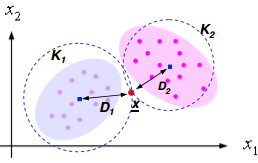
\includegraphics[width=5cm]{./images/minimum_distance_classifier.png}
        
        When the \em Mahalanobis distance \em is taken instead of the Euclidean distance, the variance is 
        also included in the min-dist-classifier:
        $$\boxed{D_j(\bm{x})^2 = (\bm x - \bm m_j)^T \bm{C}_j^{-1} (\bm x -\bm m_j)}$$
        with $\bm C_j$ as the covariance matrix for every 
        sample per class: 
        $$\bm C_j = \frac{1}{N_j} \sum_{\bm x \in K_j} \bm x \bm x^T - \bm m_j \bm m_j^T.$$
        
      \skriptsubsubsection{Matching by Correlation}{869}
        Correlation is not robust in terms of background and freeform objects (only square objects).
        
      \skriptsubsubsection{Bayes Classifier}{874}
        Binary loss function: $d_j(\bm x) = p(\bm x | K_j) p(K_j)$ ($j=1,\ldots,W$).
        $p(\bm x | K_j)$ is assumed to be Gaussian distributed:      
        $$d_j(\bm x) = \ln p(K_j)  - \frac{1}{2} \ln |\bm C_j| - \frac12 (\bm x - m_j)^T \bm C_j^{-1} (\bm x - m_j)) $$
      
      
  \end{minipage} \hspace{5mm}
  \begin{minipage}{10cm}
  
    \skriptsubsection{Neural Nets}{882}
      No assumptions about statistical model, training via samples.
      
      2-Layer perceptron for linearly separable classes
      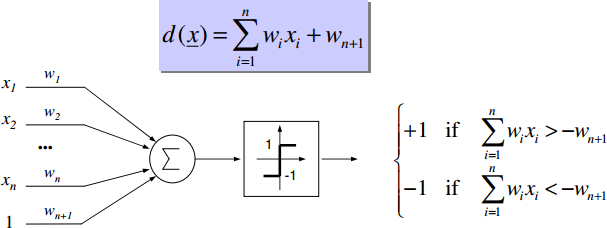
\includegraphics[width=6cm]{./images/2layer-perceptron.png}
      
      3-Layer perceptron for non-linearly separable classes with nonlinear perceptron function
      
      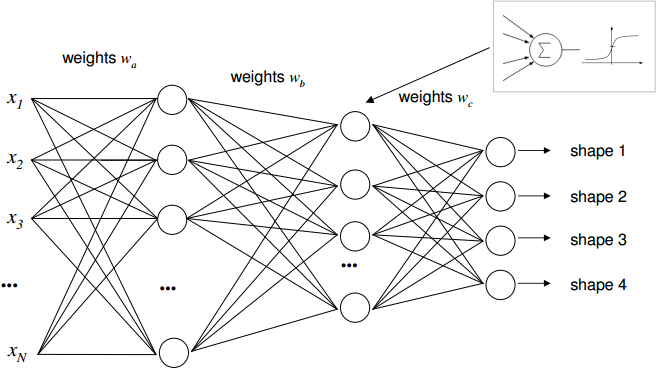
\includegraphics[width=6cm]{./images/multilayer-perceptron.png}
      
    \skriptsubsection{Structural Methods}{903}
      Classification based on common descriptors (order descriptors) according to degree of similarity:\\
      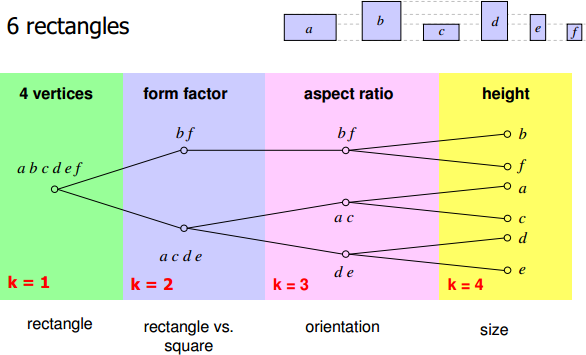
\includegraphics[width=7cm]{./images/common_features.png}\\
      Measure the similarity: Largest number to which $k$ is the same.
      Distance between two objects $a$ and $b$: $D(a,b) = \frac{1}{k}$
      
      Build similarity matrix:\\
      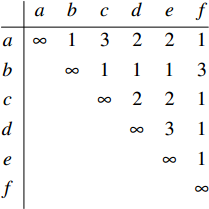
\includegraphics[width=3cm]{./images/similarity_matrix.png}
  \end{minipage}

  \skriptsubsection{Grammar}{904}
    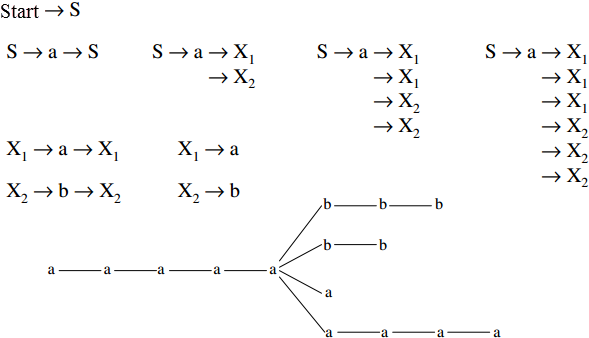
\includegraphics[width=7.5cm]{./images/grammar.png}
      